\documentclass{standalone}
\usepackage{tikz}
\usetikzlibrary{patterns, positioning}
\usepackage[sfdefault]{ClearSans} %% option 'sfdefault' activates Clear Sans as the default text font
\usepackage[T1]{fontenc}

\begin{document}
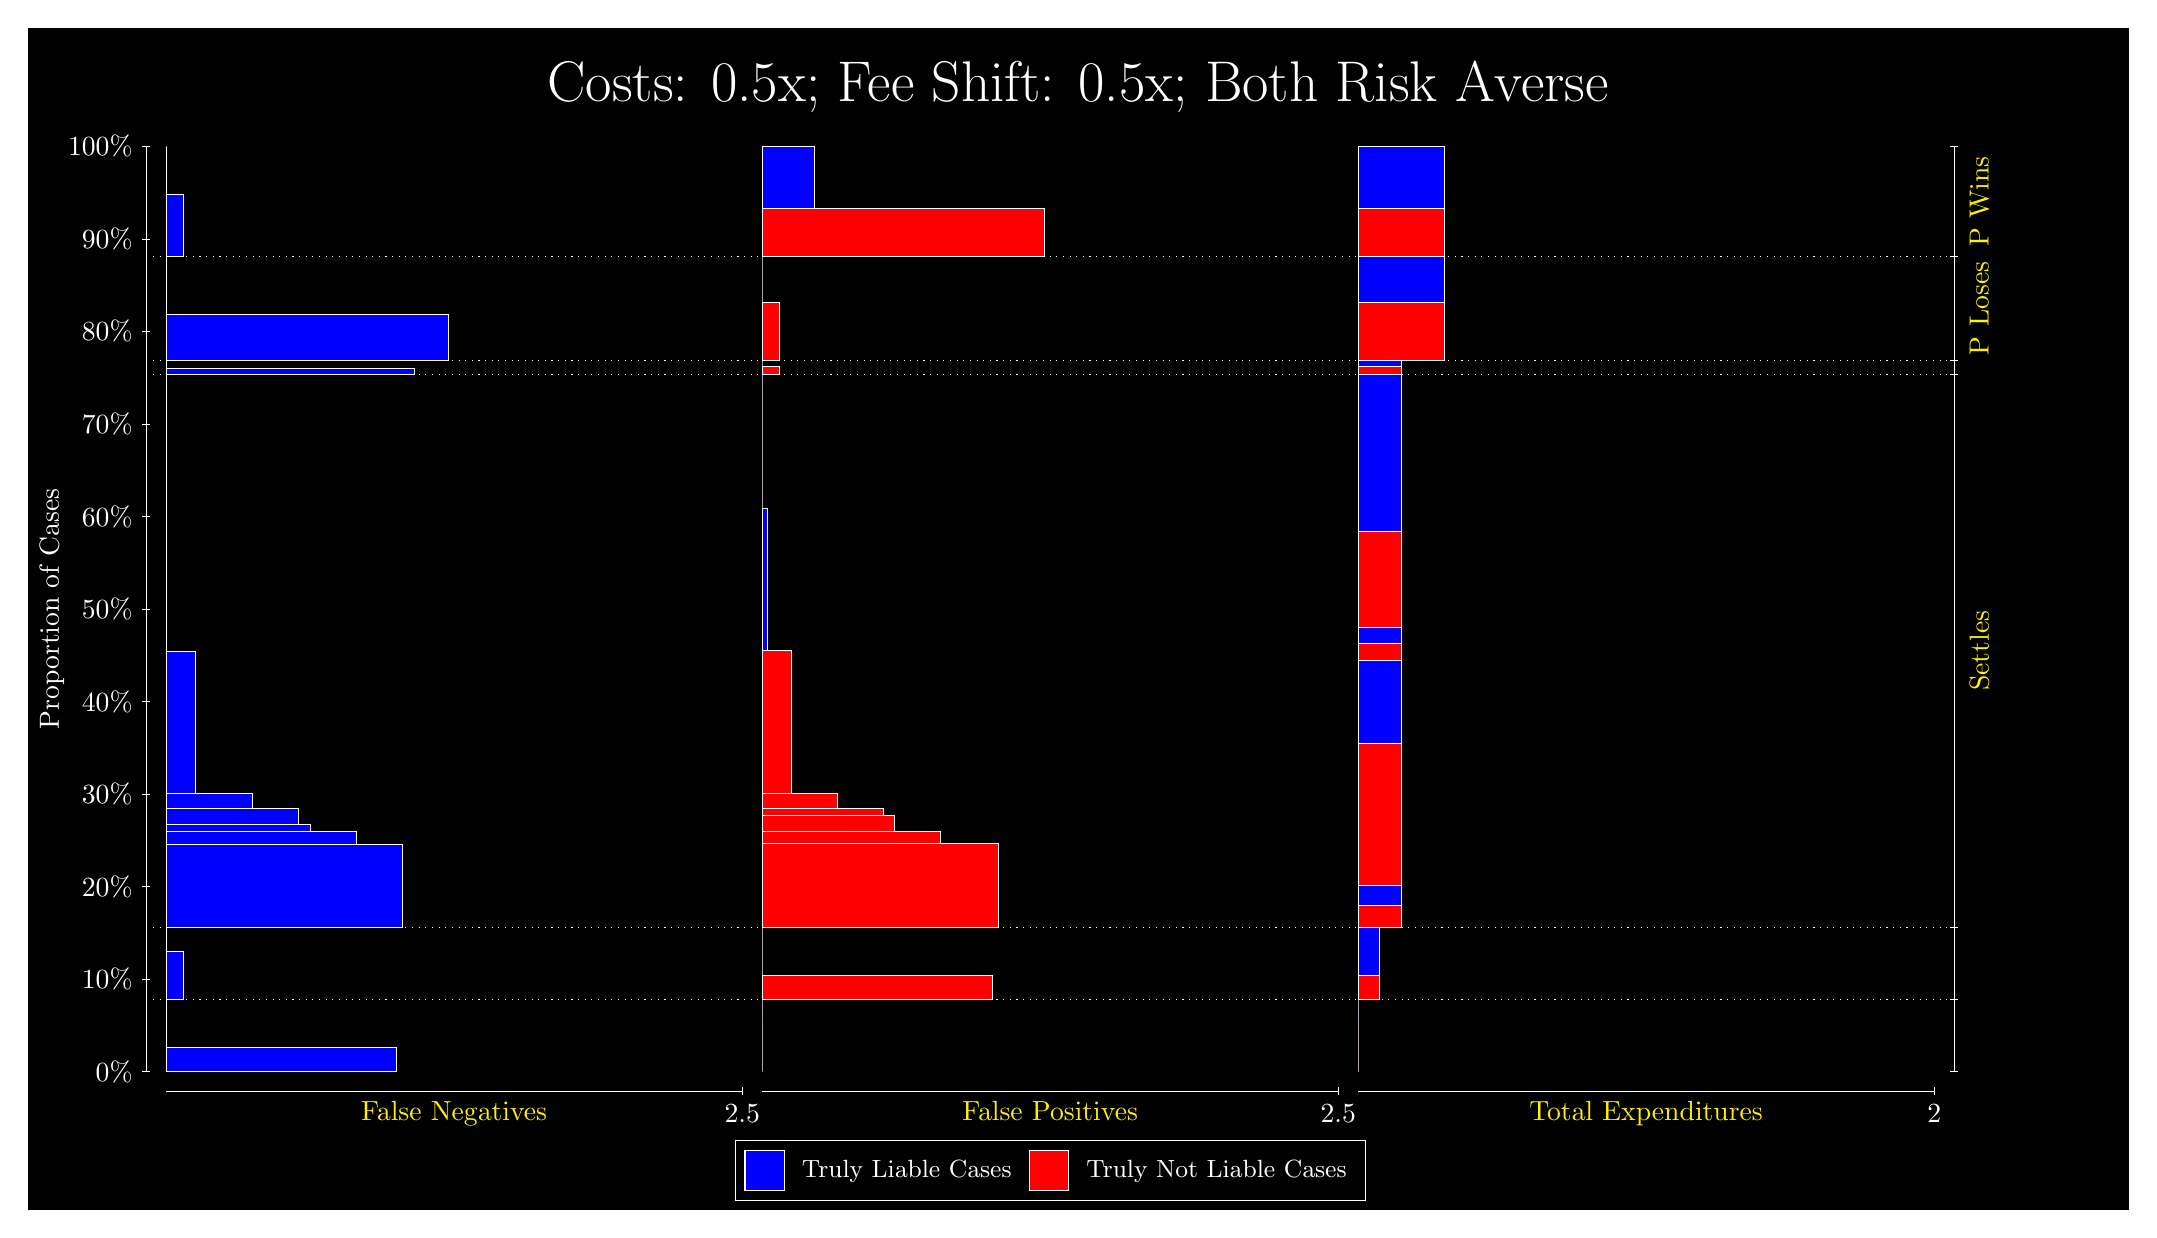
\begin{tikzpicture}
\draw[fill=black] (0,0) rectangle (26.667,15);
\draw[text=white] (0,13.5) rectangle (26.667,15) node[midway] {\huge Costs: 0.5x; Fee Shift: 0.5x; Both Risk Averse};
\draw[white, very thin] (1.5,1.75) -- (1.5,13.5);
\node[rotate=90, text=white, anchor=center] at (0.3, 7.625) {Proportion of Cases};
\draw[white, very thin] (1.45,1.75) -- (1.55,1.75);
\node[text=white, anchor=east] at (1.45, 1.75) {0\%};
\draw[white, very thin] (1.45,2.925) -- (1.55,2.925);
\node[text=white, anchor=east] at (1.45, 2.925) {10\%};
\draw[white, very thin] (1.45,4.1) -- (1.55,4.1);
\node[text=white, anchor=east] at (1.45, 4.1) {20\%};
\draw[white, very thin] (1.45,5.275) -- (1.55,5.275);
\node[text=white, anchor=east] at (1.45, 5.275) {30\%};
\draw[white, very thin] (1.45,6.45) -- (1.55,6.45);
\node[text=white, anchor=east] at (1.45, 6.45) {40\%};
\draw[white, very thin] (1.45,7.625) -- (1.55,7.625);
\node[text=white, anchor=east] at (1.45, 7.625) {50\%};
\draw[white, very thin] (1.45,8.8) -- (1.55,8.8);
\node[text=white, anchor=east] at (1.45, 8.8) {60\%};
\draw[white, very thin] (1.45,9.975) -- (1.55,9.975);
\node[text=white, anchor=east] at (1.45, 9.975) {70\%};
\draw[white, very thin] (1.45,11.15) -- (1.55,11.15);
\node[text=white, anchor=east] at (1.45, 11.15) {80\%};
\draw[white, very thin] (1.45,12.325) -- (1.55,12.325);
\node[text=white, anchor=east] at (1.45, 12.325) {90\%};
\draw[white, very thin] (1.45,13.5) -- (1.55,13.5);
\node[text=white, anchor=east] at (1.45, 13.5) {100\%};

\draw[white, very thin] (24.457,1.75) -- (24.457,13.5);
\draw[white, very thin] (24.407,1.75) -- (24.507,1.75);
\node[anchor=west] at (24.407, 1.75) {};
\draw[white, very thin] (24.407,2.6669) -- (24.507,2.6669);
\node[anchor=west] at (24.407, 2.6669) {};
\draw[white, very thin] (24.407,3.5824) -- (24.507,3.5824);
\node[anchor=west] at (24.407, 3.5824) {};
\draw[white, very thin] (24.407,10.604) -- (24.507,10.604);
\node[anchor=west] at (24.407, 10.604) {};
\draw[white, very thin] (24.407,10.782) -- (24.507,10.782);
\node[anchor=west] at (24.407, 10.782) {};
\draw[white, very thin] (24.407,12.103) -- (24.507,12.103);
\node[anchor=west] at (24.407, 12.103) {};
\draw[white, very thin] (24.407,13.5) -- (24.507,13.5);
\node[anchor=west] at (24.407, 13.5) {};

\draw[white, very thin, fill=blue] (1.75,1.75) rectangle (4.6775,2.0594);
\draw[white, very thin, fill=red] (1.75,2.0594) rectangle (1.75,2.6669);
\draw[white, very thin, fill=blue] (1.75,2.6669) rectangle (1.9696,3.2736);
\draw[white, very thin, fill=red] (1.75,3.2736) rectangle (1.75,3.5824);
\draw[white, very thin, fill=blue] (1.75,3.5824) rectangle (4.7507,4.6395);
\draw[white, very thin, fill=blue] (1.75,4.6395) rectangle (4.1652,4.795);
\draw[white, very thin, fill=blue] (1.75,4.795) rectangle (3.5797,4.8848);
\draw[white, very thin, fill=blue] (1.75,4.8848) rectangle (3.4333,5.096);
\draw[white, very thin, fill=blue] (1.75,5.096) rectangle (2.8478,5.2799);
\draw[white, very thin, fill=blue] (1.75,5.2799) rectangle (2.1159,7.0933);
\draw[white, very thin, fill=red] (1.75,7.0933) rectangle (1.75,10.604);
\draw[white, very thin, fill=blue] (1.75,10.604) rectangle (4.8971,10.68);
\draw[white, very thin, fill=red] (1.75,10.68) rectangle (1.75,10.782);
\draw[white, very thin, fill=blue] (1.75,10.782) rectangle (5.3362,11.371);
\draw[white, very thin, fill=red] (1.75,11.371) rectangle (1.75,12.103);
\draw[white, very thin, fill=blue] (1.75,12.103) rectangle (1.9696,12.886);
\draw[white, very thin, fill=red] (1.75,12.886) rectangle (1.75,13.5);
\draw[white, very thin, fill=red] (9.3189,1.75) rectangle (9.3189,2.3574);
\draw[white, very thin, fill=blue] (9.3189,2.3574) rectangle (9.3189,2.6669);
\draw[white, very thin, fill=red] (9.3189,2.6669) rectangle (12.246,2.9756);
\draw[white, very thin, fill=blue] (9.3189,2.9756) rectangle (9.3189,3.5824);
\draw[white, very thin, fill=red] (9.3189,3.5824) rectangle (12.32,4.645);
\draw[white, very thin, fill=red] (9.3189,4.645) rectangle (11.588,4.7949);
\draw[white, very thin, fill=red] (9.3189,4.7949) rectangle (11.002,5.0061);
\draw[white, very thin, fill=red] (9.3189,5.0061) rectangle (10.856,5.0963);
\draw[white, very thin, fill=red] (9.3189,5.0963) rectangle (10.27,5.2877);
\draw[white, very thin, fill=red] (9.3189,5.2877) rectangle (9.6848,7.0936);
\draw[white, very thin, fill=blue] (9.3189,7.0936) rectangle (9.3921,8.907);
\draw[white, very thin, fill=blue] (9.3189,8.907) rectangle (9.3189,10.604);
\draw[white, very thin, fill=red] (9.3189,10.604) rectangle (9.5384,10.706);
\draw[white, very thin, fill=blue] (9.3189,10.706) rectangle (9.3189,10.782);
\draw[white, very thin, fill=red] (9.3189,10.782) rectangle (9.5384,11.514);
\draw[white, very thin, fill=blue] (9.3189,11.514) rectangle (9.3189,12.103);
\draw[white, very thin, fill=red] (9.3189,12.103) rectangle (12.905,12.717);
\draw[white, very thin, fill=blue] (9.3189,12.717) rectangle (9.9776,13.5);
\draw[white, very thin, fill=red] (16.888,1.75) rectangle (16.888,2.3574);
\draw[white, very thin, fill=blue] (16.888,2.3574) rectangle (16.888,2.6669);
\draw[white, very thin, fill=red] (16.888,2.6669) rectangle (17.162,2.9756);
\draw[white, very thin, fill=blue] (16.888,2.9756) rectangle (17.162,3.5824);
\draw[white, very thin, fill=red] (16.888,3.5824) rectangle (17.437,3.864);
\draw[white, very thin, fill=blue] (16.888,3.864) rectangle (17.437,4.1093);
\draw[white, very thin, fill=red] (16.888,4.1093) rectangle (17.437,5.9152);
\draw[white, very thin, fill=blue] (16.888,5.9152) rectangle (17.437,6.9724);
\draw[white, very thin, fill=red] (16.888,6.9724) rectangle (17.437,7.1835);
\draw[white, very thin, fill=blue] (16.888,7.1835) rectangle (17.437,7.3947);
\draw[white, very thin, fill=red] (16.888,7.3947) rectangle (17.437,8.6072);
\draw[white, very thin, fill=blue] (16.888,8.6072) rectangle (17.437,10.604);
\draw[white, very thin, fill=red] (16.888,10.604) rectangle (17.437,10.706);
\draw[white, very thin, fill=blue] (16.888,10.706) rectangle (17.437,10.782);
\draw[white, very thin, fill=red] (16.888,10.782) rectangle (17.986,11.514);
\draw[white, very thin, fill=blue] (16.888,11.514) rectangle (17.986,12.103);
\draw[white, very thin, fill=red] (16.888,12.103) rectangle (17.986,12.717);
\draw[white, very thin, fill=blue] (16.888,12.717) rectangle (17.986,13.5);
\draw[white, dotted] (1.5,2.6669) -- (24.457,2.6669);
\draw[white, dotted] (1.5,3.5824) -- (24.457,3.5824);
\draw[white, dotted] (1.5,10.604) -- (24.457,10.604);
\draw[white, dotted] (1.5,10.782) -- (24.457,10.782);
\draw[white, dotted] (1.5,12.103) -- (24.457,12.103);
\draw[white, very thin] (1.75,1.5) -- (9.0689,1.5);
\node[text=yellow, anchor=north] at (5.4094, 1.5) {False Negatives};
\draw[white, very thin] (9.0689,1.45) -- (9.0689,1.55);
\node[text=white, anchor=north] at (9.0689, 1.45) {2.5};

\draw[white, very thin] (9.3189,1.5) -- (16.638,1.5);
\node[text=yellow, anchor=north] at (12.978, 1.5) {False Positives};
\draw[white, very thin] (16.638,1.45) -- (16.638,1.55);
\node[text=white, anchor=north] at (16.638, 1.45) {2.5};

\draw[white, very thin] (16.888,1.5) -- (24.207,1.5);
\node[text=yellow, anchor=north] at (20.547, 1.5) {Total Expenditures};
\draw[white, very thin] (24.207,1.45) -- (24.207,1.55);
\node[text=white, anchor=north] at (24.207, 1.45) {2};



\node[text=yellow, centered, rotate=90] at (24.777, 7.0934) {Settles};

\node[text=yellow, centered, rotate=90] at (24.777, 11.442) {P Loses};
\node[text=yellow, centered, rotate=90] at (24.777, 12.801) {P Wins};

\draw (12.978300999999998,1.5) node[draw=none] (baseCoordinate) {};
\begin{scope}[align=center]
        \matrix[scale=0.5, draw=white, below=0.5cm of baseCoordinate, nodes={draw}, column sep=0.1cm]{
            \node[rectangle, draw, minimum width=0.5cm, minimum height=0.5cm, fill=blue] {}; &
            \node[draw=none, font=\small, text=white] (B) {Truly Liable Cases}; &
            \node[rectangle, draw, minimum width=0.5cm, minimum height=0.5cm, fill=red] {}; &
            \node[draw=none, font=\small, text=white] (B) {Truly Not Liable Cases}; \\
            };
\end{scope}

\end{tikzpicture}
\end{document}